\chapter{On Sampled Metrics for Item Recommendation}

Google Research \\

\textbf{Best research paper award}

\textbf{Reference:}~\url{http://walid.krichene.net/papers/KDD-sampled-metrics.pdf}

\textbf{Keywords:} ranking evaluation, metrics, sampling

\section*{Какую задачу решают авторы?}

Типичный протокол оценки качества рекомендательных систем выглядит следующим образом:
\begin{enumerate}
    \item Для отобранного множества пользователей $D$ ранжируем алгоритмом $A$ все множество кандидатов, состоящее из $n$ объектов
    \item Для каждого пользователя $\vecx$ вычисляем $R(A, \vecx)$ --- множество позиций релевантных объектов
    \item После чего для пользователя считаем метрику $M$, например, \texttt{ROC AUC} или \texttt{Precision@K}, \texttt{Recall@K}
\end{enumerate}

Итоговое значение метрики получается усредненеим метрик посчитанных по всем пользователям
\begin{equation*}
    \frac{1}{|D|}\sum\limits_{\vecx \in D} M(R(A, \vecx)) .
\end{equation*}

В ситуации когда $n$ велико часто прибегают к сэмплированию --- вместо того чтобы ранжировать все $n$ кандидатов, ранжируют случайную подвыборку из $m$ объектов ($ m \ll n $) вместе с релевантными для пользователя объектами. \\

Ожидается, что метрики посчитанные с сэмплированием позволяют упорядочить алгоритмы ранжирования по качеству так же как и метрики посчитанные без сэмплирования. 

Авторы статьи впервые тестируют это предположение и показывают что для большинства используемых метрик оно не верно, даже при многократном сэмплировании и усреднении результатов. \\

В статье предложены скорректированные варианты привычных метрик, которые позволяют при использовании сэмплирования сортировать алгоритмы по качеству также как если бы сэмплирования не было. 

\section*{Как решают?}

\textbf{Remark:} для простоты можно считать, что для каждого пользователя есть один релевантный объект. \\

Работу можно разбить на три части
\begin{enumerate}
    \item Экспериментальная часть, где проверяют предположение, что метрики с сэмплированием и без упорядочивают алгоритмы ранжирования одинаковым образом
    \item Теоретическая часть, посвященная скорректированным вариантам метрик
    \item Экспериментальная часть, где авторы показывают, что скорректированные варианты метрик работают
\end{enumerate}

\subsection*{Inconsistency of Sampled Metrics}

Ключевое определение данной работы

\ddef{Consistency}{
\label{def:consistenct}
Let the evaluation data $D$ be fixed. A metric $M$ is consistent under sampling if the relative order of any two recommenders $A$ and $B$ is preserved in expectation. That is, for all $A,B$,
\begin{align*}
    & \frac{1}{|D|} \sum\limits_{\vecx \in D} M(R(A,\vecx)) > \frac{1}{|D|} \sum\limits_{\vecx \in D} M(R(B,\vecx)) \\
    \Longleftrightarrow & \bE \left[ \frac{1}{|D|} \sum\limits_{\vecx \in D} M(\widetilde{R}(A,\vecx))  \right] > \bE \left[ \frac{1}{|D|} \sum\limits_{\vecx \in D} M(\widetilde{R}(B,\vecx))  \right]
\end{align*}
}

В рамках первой группы экспериментов (см. Рисунок~\ref{fig:example_vary_m}) показывают как меняются метрики для разных алгоритмов в зависимости от $m$ (число случайно отобранных объектов). \\

\begin{figure}[ht]
    \centering
    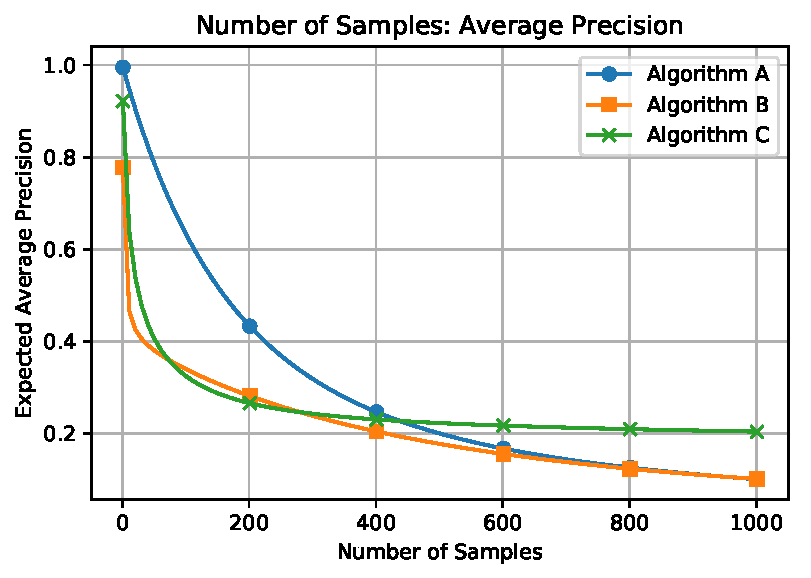
\includegraphics[width=0.49\textwidth]{figures/ex_num_samples_vs_ap.pdf}
    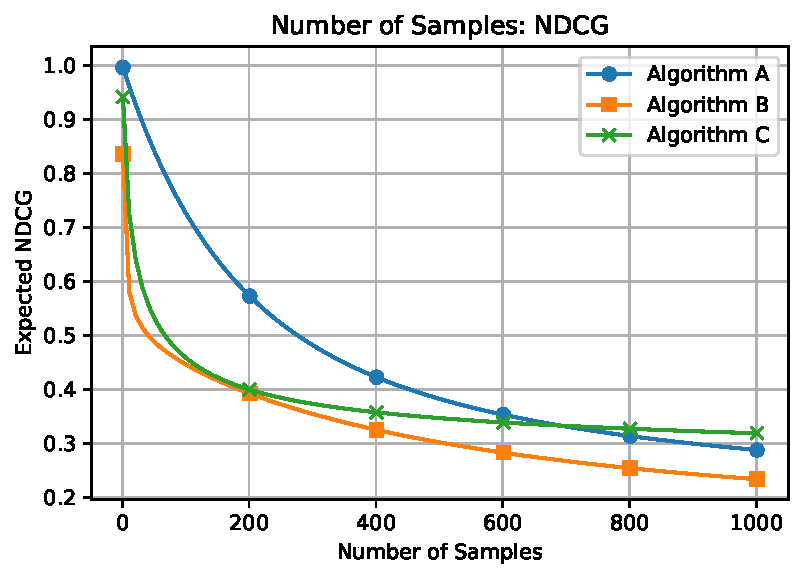
\includegraphics[width=0.49\textwidth]{figures/ex_num_samples_vs_ndcg.pdf} \newline
    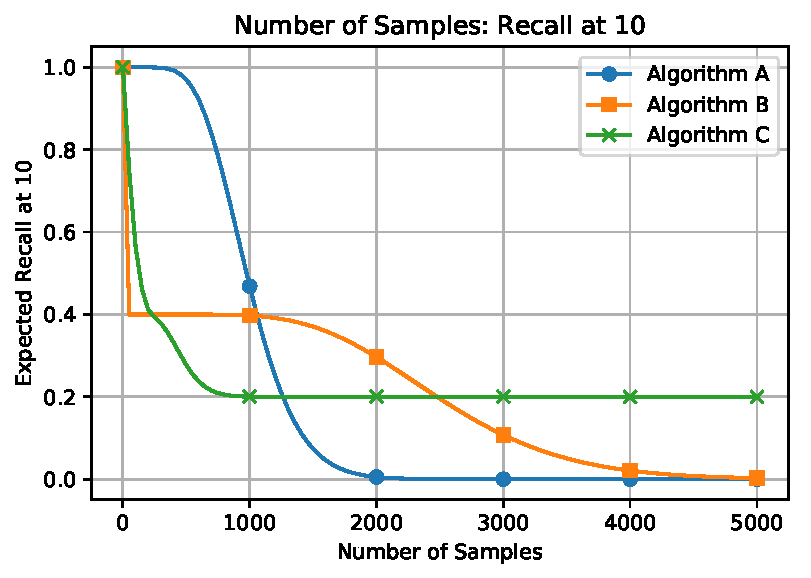
\includegraphics[width=0.49\textwidth]{figures/ex_num_samples_vs_recall.pdf}
    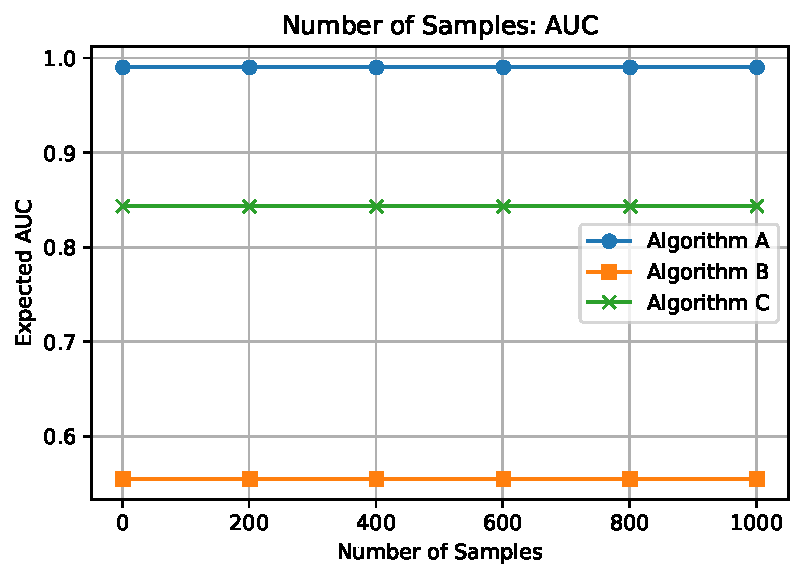
\includegraphics[width=0.49\textwidth]{figures/ex_num_samples_vs_auc.pdf}
    \caption{\footnotesize{Expected sampling metrics for the running example while increasing the number of samples.
    For Average Precision, NDCG and Recall, even the relative order of algorithm performance changes with the number of samples.
    That means, conclusions drawn from a subsample are not consistent with the true performance of the algorithm.}}
    \label{fig:example_vary_m}
\end{figure}

Из экспериментов видно, что единственная консистентная метрика --- \texttt{ROC AUC}.

\subsection*{Corrected Metrics}

Очень рекомендую самостоятельно ознакомиться с данной частью работы, так как ее не очень удобно излогать в виде конспекта.

\section*{Выводы}

\dbox{\textbf{Key Takeaways}:
\begin{enumerate}
    \item Нужно избегать сэмплирования при расчете метрик
    \item Если нет возможности избежать сэмплирования, то нужно использовать скорректированные версии метрик
    \item Вычисление метрик нужно повторять несколько раз с разным seed'ом для того чтобы уменьшить дисперсию
\end{enumerate}}

Все это в лишний раз наводит на мысли о том, что в ряде работ лучшими оказались алгоритмы, которые не обязательно являются лучшими на самом деле, и на результаты экспериментов в статьях всегда надо смотреть с определенной долей скепсиса. \\

Еще одна работа примерно про тоже On Sampling Top-K Recommendation Evaluation~\url{https://dl.acm.org/doi/pdf/10.1145/3394486.3403262} с этой же конференции.